    % THIS IS SIGPROC-SP.TEX - VERSION 3.1
% WORKS WITH V3.2SP OF ACM_PROC_ARTICLE-SP.CLS
% APRIL 2009
%
% It is an example file showing how to use the 'acm_proc_article-sp.cls' V3.2SP
% LaTeX2e document class file for Conference Proceedings submissions.
% ----------------------------------------------------------------------------------------------------------------
% This .tex file (and associated .cls V3.2SP) *DOES NOT* produce:
%       1) The Permission Statement
%       2) The Conference (location) Info information
%       3) The Copyright Line with ACM data
%       4) Page numbering
% ---------------------------------------------------------------------------------------------------------------
% It is an example which *does* use the .bib file (from which the .bbl file
% is produced).
% REMEMBER HOWEVER: After having produced the .bbl file,
% and prior to final submission,
% you need to 'insert'  your .bbl file into your source .tex file so as to provide
% ONE 'self-contained' source file.
%
% Questions regarding SIGS should be sent to
% Adrienne Griscti ---> griscti@acm.orghttps://www.overleaf.com/7267312825nsgbbwvhhrxchttps://www.overleaf.com/7267312825nsgbbwvhhrxc
%
% Questions/suggestions regarding the guidelines, .tex and .cls files, etc. to
% Gerald Murray ---> murray@hq.acm.org
%
% For tracking purposes - this is V3.1SP - APRIL 2009

\documentclass{edm_template}


\usepackage{tikz}
\usetikzlibrary{bayesnet}
\usetikzlibrary{arrows}
\usepackage{enumitem}
\usepackage{amsmath}
\usepackage{mathtools}

\DeclarePairedDelimiterX{\infdivx}[2]{(}{)}{%
  #1\;\delimsize\|\;#2%
}


\usepackage{hyperref}
\newcommand{\infdiv}{D_{KL}\infdivx}

% \usepackage[dvipsnames]{xcolor}

% \providecommand{\am}[1]{{\color{blue} [AM: #1]}}
% \providecommand{\nvg}[1]{{\color{red} [NG: #1]}}
% \providecommand{\bc}[1]{{\color{orange} [BC: #1]}}
% \providecommand{\piech}[1]{{\color{purple}{[cjp: #1]}}}
% \providecommand{\ms}[1]{{\color{magenta}{[MS: #1]}}}


% \providecommand{\am}[1]{{\color{blue} }}
% \providecommand{\nvg}[1]{{\color{red} }}
% \providecommand{\bc}[1]{{\color{orange} }}
% \providecommand{\piech}[1]{{\color{purple}{}}}
% \providecommand{\ms}[1]{{\color{magenta}{}}}

\begin{document}

\title{Latent Variable Models of Enrollment for Course Planning and Understanding}

\numberofauthors{6} %  in this sample file, there are a *total*
% \author{
% \alignauthor Anonymous Authors \\
%       \affaddr{Anonymous Universities}\\
%       \email{anon@anonymous.com}
% }
\author{
\alignauthor Nate Gruver \\
      \affaddr{Stanford University}\\
      \email{ngruver@cs.stanford.edu}
\alignauthor Ali Malik \\
      \affaddr{Stanford University}\\
      \email{malikali@cs.stanford.edu}
\alignauthor Brahm Capoor \\
      \affaddr{Stanford University}\\
      \email{brahm@cs.stanford.edu}
\and
\alignauthor Chris Piech\\
      \affaddr{Stanford University}\\
      \email{piech@cs.stanford.edu}
\alignauthor Mitchell Stevens\\
      \affaddr{Stanford University}\\
      \email{stevens4@stanford.edu}
\alignauthor Andreas Paepcke \\
      \affaddr{Stanford University}\\
      \email{paepcke@cs.stanford.edu}
}
% There's nothing stopping you putting the seventh, eighth, etc.
% author on the opening page (as the 'third row') but we ask,
% for aesthetic reasons that you place these 'additional authors'
% in the \additional authors block, viz.

% Just remember to make sure that the TOTAL number of authors
% is the number that will appear on the first page PLUS the
% number that will appear in the \additionalauthors section.

\maketitle
\begin{abstract}

Understanding large-scale patterns in student course enrollment is a problem of great interest to university administrators and educational researchers. Despite this, impactful decisions are often made without a good quantitative framework of the process underlying student choices. We propose a probabilistic approach to modelling course enrollment decisions, drawing inspiration from natural language processing and mixture models. We use 10 years of anonymised student transcripts from a large university to construct a Gaussian latent variable model that learns the joint distribution over course enrollments. Such models are generative in nature, allowing for a diverse set of inference queries and robustness to data sparsity. We demonstrate the efficacy of this model in comparison to other approaches---including deep learning architectures---and show that it is able to capture underlying student interests that guide enrollment decisions. 
\end{abstract}

%% A category with the (minimum) three required fields
%\category{H.4}{Information Systems Applications}{Miscellaneous}
%%A category including the fourth, optional field follows...
%\category{D.2.8}{Software Engineering}{Metrics}[complexity measures, performance measures]
%
%\terms{Theory}

\keywords{Enrollment modeling, Mixture models, Hidden Markov Model, Latent Dirichlet Allocation, Post-secondary education} % NOT required for Proceedings

\section{Introduction}

\begin{figure*}
    \centering
    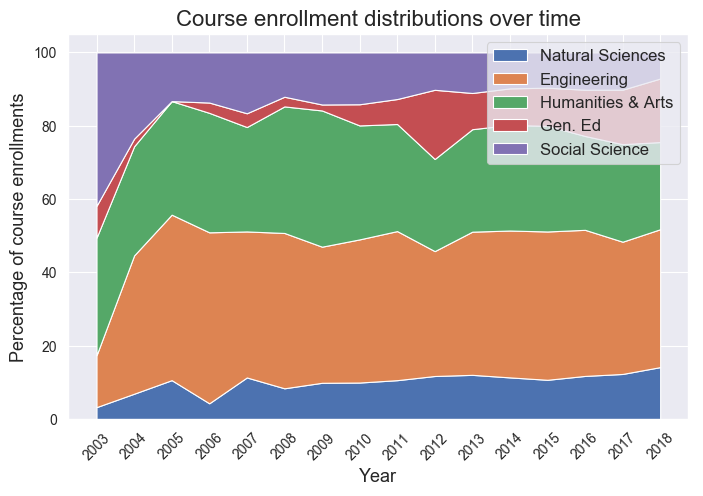
\includegraphics[scale=0.48]{figures/dists_over_time.png}
    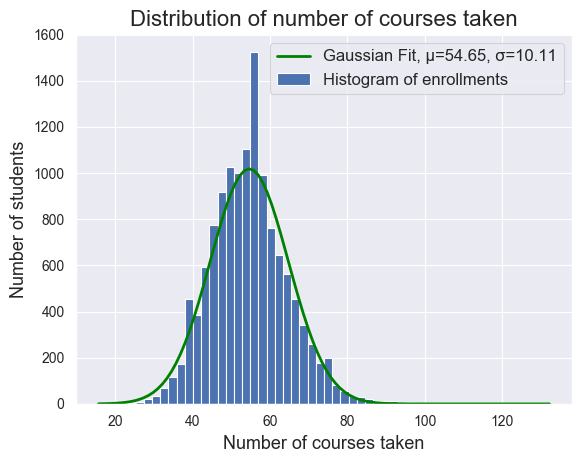
\includegraphics[scale=0.51]{figures/enrollment_dist.png}
    \caption{Top: A stacked area plot of enrolled courses per university sub-school per year. Bottom: A histogram of the number of courses taken by each individual student with a Gaussian fitting.}
    \label{fig:data_statistics}
\end{figure*}

Understanding the enrollment decisions of students in post-secondary institutions is central to the success of university administrators, researchers, and advisors. Despite this, students and staff rely primarily on heuristics, word-of-mouth, or complex mental models for the bulk of course planning. Although much work has been devoted to predicting course enrollments and collaborative filtering for course planning, few studies have attempted to computationally model the robust framework that experienced students develop. Such a model is not just discriminative, but is also capable of counterfactual thinking, inferring intentions, or detecting anomalies in course planning.

To handle these more nuanced tasks, we propose a fully generative model of course enrollment. The distinguishing feature of a generative model is its ability to describe the full joint distribution over the feature space: in our case a student's binary-valued course enrollments. This increased expressiveness makes it possible to ask powerful inference queries---for example how likely it is for a student to take course X conditioned on their past enrollments. Importantly, since the model captures the joint distribution, it is possible to draw samples from the model. This allows us to determine likely upcoming course choices based on the trained model's observations of all students' past choices.

The probabilistic nature of the generative model we propose is a promising foundation for future course selection and student advising support facilities. For example, given an advising application built atop our model, advisers could evaluate how unusual a given student's proposed next-course choice would be, compared to paths that others have chosen in the past. Such insights could alert the advisor to pay extra attention to possible conflicts in major requirements, or the student's underestimation of workload.

A use case for students themselves would be a tool that recommends course choice paths towards a goal. The student could specify how much the suggestions should match ``mainstream'' choices, versus more unusual course tangents. While we have not implemented such an application, the model construction we propose here enables their construction.

Somewhat more formally, these examples can be expressed in probabilistic terms as follows:

\begin{itemize}[noitemsep,topsep=0pt]
	\item A student prototyping their set of future enrollments based on common paths, i.e. queries of the form
	$$P(\text{Enrollment}_t \mid \text{Enrollment}_{1,..,t-1})$$ 
	\item An advisor wondering if their advisee is on track, i.e. queries of the form
	$$P(\text{Student's enrollment} \mid \text{All other student enrollments})$$
    \item An administrator trying to ascertain the popular paths through a major, with queries of the form
	$$\arg\max_{V} P(\text{Path} = V | \text{All enrollments})$$.
\end{itemize}

These motivating examples represent a small subset of the possible enrollment queries relevant to the operations of a university. Rather, they simply give a taste for how such questions can be framed in probabilistic language and then answered with the model presented here. 

\subsection{Prior Work}
\label{section:related-work}

Much of the prior work on enrollment modeling in the university setting is dedicated purely to predictive models, both of future course enrollment \cite{kardan2013prediction}\cite{nandeshwar2009enrollment}\cite{song1993new} and academic performance \cite{kovacic2010early}\cite{hlosta2017ouroboros}. 
% \bc{Weird segue between this next sentence and the last}
% Among the most compelling of these approaches is Kardan et al.'s use of a neural network trained on hand-selected features to predict the probability of a future enrollment \cite{kardan2013prediction}. 
Most state-of-the-art research in student decision modeling is now found in the study of massive open online courses (MOOCs). Studies of students in these courses range in their focus from tracking student engagement to predicting future decisions and success. Gardner and Brooks \cite{Gardner2018StudentSP} provide a thorough overview of modern models for the problem, but we investigate two relevant approaches here. Balakrishnan and Coetzee use a Hidden Markov Model (HMM) to predict attrition in MOOCs by modeling the probability of a binary drop/no-drop decision per timestep \cite{balakrishnan2013predicting}. Similarly, Al-Shabandar et al. use Gaussian Mixture Models (GMMs) to cluster MOOC students at each timestep, and thus identify clusters of students that are likely to withdraw from the courses  \cite{AlShabandar2018TheAO}. Both of these models are highly related to our approach as they use graphical models to model student decisions. Their priority, however, is prediction of simple binary outcomes. In contrast, we seek to model the complex interactions of many courses jointly.

Another related body of work focuses on course recommender systems, which often leverage enrollment prediction as a subsystem, along with more sophisticated models of intention. Khorasani et al create a fully-observed Markov model of course enrollment sequences, estimating the probability of taking a course after others via maximum likelihood estimation (MLE)~\cite{Khorasani2016AMC}. Their use of a sequential probabilistic model parallels ours, but our use of latent variables gives us the added benefit of robustness to cases in which maximum likelihood is weak---namely when there are few examples of some enrollment patterns or when the number of variables being modeled jointly grows large. Jiang et al. achieve a similar level of sophistication in their neural-network based course recommender system~\cite{Jiang2018GoalbasedCR}, which uses predictions of grade outcomes to create custom course recommendations. Instead of a fully probabilistic model, they employ a recurrent neural network (RNN) that uses past semesters as inputs for the predictions (also see~\cite{pardos2018connectionist}). Although this model yields compelling results, it is not capable of the broad range of inference queries possible with our model. The most immediate limitation is in its ability to reason backwards in time, estimating probabilities on earlier states given future ones. 

A final significant branch of enrollment modeling research in the university setting does not prioritize prediction, but instead focuses on clustering courses for the purpose of understanding the semantic landscape of a university. These studies relate to the work here insofar as they seek to discover relationships between courses. Some authors focus on clustering courses \cite{Motz2018FindingTI}\cite{Pardos2018AMO} while others focus instead on students~\cite{Zeidenberg2011TheCO}\cite{Slim2016TheIO}. The two common approaches for clustering courses are latent variable models like Latent Dirichlet Allocation (LDA) used by Motz et al. and Recurrent Neural Networks (RNNs) as used by Pardos et al.. In our work, we directly consider both deep learning and simpler latent variable models like LDA and use these models as comparisons for our model. Among the authors that focus more directly on clustering students, Zeidenberg primarily defines distance metrics~\cite{Zeidenberg2011TheCO} over students, and Slim et al. present feature extraction approaches using graph operations~\cite{Slim2016TheIO}. 

The primary limitation of the prior work is a lack of flexibility. Strong predictive models can be trained, but they are discriminative instead of generative and thus lack the ability to answer nuanced inference queries. Adopting the more general probabilistic approach presented here opens the door for a much more diverse set of analyses within a shared statistical framework.

\section{Background \& Models}
\label{section:background}

There is a rich history of using probabilistic graphical models (PGMs) in the study of natural language. Conveniently, natural language processing (NLP) shares many characteristics with the enrollment modeling task at hand. First, both concern categorical and sequentially structured data. Second, both enrollments and natural language tokens can be understood as the observable counterpoints to mostly unobserved semantic intentions. Noting these similarities, we utilize models that have been successful in NLP. Specifically, we analogize enrollments as natural language tokens, and students as the documents comprising these enrollments. We employ latent variable models in our analysis because of their ability to capture unseen factors that influence the observed data. In the case of student course enrollments, these latent variables might correspond to the underlying typography of students such as their personal interests or underlying motiviations behind taking certain courses.

\subsection{Latent Variable Models}
\label{section:latent-variable-models}

Latent variable models are a subclass of PGMs in which some variables are never observed in training data and are thus ``latent". These models are typically computationally demanding because of the marginalization required to calculate probabilities without fixed assignments to these hidden variables. They also, however, allow us to learn potentially complex structure in data without supervision. 

\subsubsection{Latent Dirichlet Allocation}
Among the simplest and most commonly used latent variable models is Latent Dirichlet allocation (LDA)---used for clustering of natural language documents~\cite{blei2003latent}. In this model, a latent variable captures the topics that could be present in a document, and words are drawn from a distribution conditioned on this topic. A slightly simplified version of LDA could be described with the generative process below:
\begin{align*}
\theta &\sim \text{Dir}(\alpha) \\
\text{ topic } z_i &\sim \text{Multinomial}(\theta) \\
\text{ word } w \mid z_i &\sim \text{Multinomial}(\beta) \\ 	
\end{align*}
\vspace{-11mm}

The idea is that documents are comprised of a number of topics, where each topic characterizes a distribution over words. Therefore, to generate a document, a topic distribution is sampled from a prior, and then topics are sampled from this distribution. Words are then sampled conditioned on these topics.

One obvious drawback of this model is its assumption that words are drawn independently given the selected topics. In the case of course enrollments, this is problematic for at least two reasons: firstly, because enrollment decisions often influence one another, and secondly, because the number of courses taken by students in any given year is stochastic and depends on the other courses taken. It is easier to capture these two facets of the data if we can model enrollments jointly.

\subsubsection{Gaussian Mixture Model}
Take $X_i$ to be set of enrollments for a student $i$ with 
$$X_{ij} = 
\begin{cases}
\,\,1 & $student $ i $ took class $ j \\
-1 & $otherwise$
\end{cases}
$$
Any joint probability distribution over all discrete combinations of $X_i \in \{-1,1\}^m$ would require $2^m - 1$ parameters to specify and is thus impractical. We can, however, relax the discrete problem to a real-valued vector space with $\bar{X}_i \in \mathbb{R}^m$ and $X_{ij} = \text{sign}(\bar{X}_{ij})$. With this alternative encoding of enrollments we can take advantage of real-valued distributions with much smaller parameter spaces. 

The Gaussian Mixture Model (GMM) is an archetypal latent variable model for real-valued data. Much like LDA, there is a latent variable intended to capture semantics and an emission model specifying the probability of the observed features conditioned on the latent variable. In particular, we can describe a GMM by generative process below:
\begin{align*}
h_i &\sim \text{Multinomial}(\theta) \\
\bar{X} \mid h_i &\sim \mathcal{N}(\mu_i, \Sigma_i) \\
\end{align*}
\vspace{-11mm}

A graphical representation of the mixture model with hidden categorical variable $h$ and observed enrollment vector $\bar{X}$ is also shown in Figure \ref{fig:mixture_model}. At face value it might seem odd to model enrollments as distributed according to a Gaussian, but there are at least two convincing ways to view this choice. First, we can note that a Gaussian is simply encoding an assumption of smoothness around a modal assignment. In our case that will be the modal set of enrollments corresponding to a certain cluster of students. Smoothness will describe the way that most students in this cluster will be drawn from the same mold with small variations being most common. Another convincing way to view the choice of a Gaussian follows the Central Limit Theorem, which shows that the averaged stochastic individual choices of a student tends towards a multivariate normal in the limit.

\begin{figure}
	\centering
	\tikz{
	% nodes
	\node[obs] (X0) {$X_i$};%
	\node[latent,above=of X0] (h0) {$h_i$}; %
	\node[latent,rectangle,left=of h0] (theta0) {$\theta$}; %
	\node[latent,rectangle,left=of X0] (params0) {$\mu_k, \Sigma_k$}; %
	
	\node[latent,rectangle,right=1.5cm of X0] (params1) {$\mu_k, \Sigma_k$}; %
  	\node[latent,rectangle,right=1.5cm of h0] (theta1) {$\theta, \phi$}; %
	
	\node[obs,right=of params1] (X1) {$X^t_i$};%
	\node[latent,above=of X1] (h1) {$h^t_i$}; %
	
	% plate
	\plate [inner sep=.25cm,yshift=.2cm] {plate0} {(X0)(h0)} {$N$}; %
	\plate [inner sep=.25cm,yshift=.2cm] {plate1} {(X1)(h1)} {$N$}; %
	\plate [inner sep=.25cm,yshift=.2cm] {plate2} {(params0)} {$K$}; %
	\plate [inner sep=.25cm,yshift=.2cm] {plate3} {(params1)} {$K$}; %
	
	% edges
	\edge {h0} {X0}  
	\edge {theta0} {h0}
	\edge {params0} {X0}
	
	\edge {h1} {X1}
    \edge {theta1} {h1}
	\edge {params1} {X1}
	\draw (h1) edge[loop above] node {} (h1)}
	\caption{\label{fig:mixture_model} Graphical representation of mixture model (left) and hidden Markov model (right) using plate notation}
\end{figure}

\pagebreak
\subsubsection{Contextual Mixture Model}
\label{section:cmm}

Hidden Markov Models (HMMs) are a common extension of the stationary mixture models to sequential data (Figure~\ref{fig:mixture_model})~\cite{rabiner1989tutorial}. In these models the single latent variable is replaced with a Markov chain of hidden states, with future states influenced by the previous one. This model is naturally recursive, a property that is extremely useful when modeling processes that are positive recurrent. However, as enrollments often exhibit a strict order and returning to previous states is unlikely, we prefer a model that is strictly time-dependent, or as we shall call it here ``contextual". In general any ``Contextual" Mixture Model (CMM) can be expressed using a Hidden Markov model, but enforcing this structure allows us to incorporate priors that significantly improve the chances of training a plausible model.

For a general HMM with Gaussian emission probabilities, we have 
\begin{align*}
h^0 &\sim \text{Multinomial}(\theta) \\    
h^{t+1} \mid h^{t} &\sim \text{Multinomial}(\phi) \\
x^{t} \mid h_i^{t} &\sim \mathcal{N}(\mu_i, \Sigma_i)
\end{align*}
In contrast, for a CMM we have 
\begin{align*}
h^0 &\sim \text{Multinomial}(\theta) \\    
h^{t+1} \mid h^{t} &\sim \text{Multinomial}(\phi^t) \\
x^{t} \mid h_i^{t} &\sim \mathcal{N}(\mu^t_i, \Sigma^t_i)
\end{align*}
Note that the parameters of the transition and emission distributions are different for each timestep. Figure~\ref{fig:contextual_mixture_model} shows a diagram of our proposed model in plate notation.

\begin{figure}
    \centering
	\tikz{
	% nodes
	\node[obs] (X0) {$X^0_i$};%
	\node[latent,above=of X0] (h0) {$h^0_i$}; %
	\node[latent,rectangle,above=of h0] (theta0) {$\theta$}; %
	\node[latent,rectangle,below=of X0] (params0) {$\mu^0, \Sigma^0$}; %	
	
	\node[obs,right=of X0] (X1) {$X^1_i$};%
	\node[latent,above=of X1] (h1) {$h^1_i$}; %
	\node[latent,rectangle,above=of h1] (theta1) {$\phi^1$}; %
	\node[latent,rectangle,below=of X1] (params1) {$\mu^1, \Sigma^1$}; %	
	
	\node[obs,right=of X1] (X2) {$X^2_i$};%
	\node[latent,above=of X2] (h2) {$h^2_i$}; %
	\node[latent,rectangle,above=of h2] (theta2) {$\phi^2$}; %
	\node[latent,rectangle,below=of X2] (params2) {$\mu^2, \Sigma^2$}; %	

	\node[obs,right=of X2] (X3) {$X^3_i$};%
	\node[latent,above=of X3] (h3) {$h^3_i$}; %
	\node[latent,rectangle,above=of h3] (theta3) {$\phi^3$}; %
	\node[latent,rectangle,below=of X3] (params3) {$\mu^3, \Sigma^3$}; %	
	
	% plate
	\plate [inner sep=.25cm,yshift=.2cm] {plate0} {(X0)(X1)(X2)(X3)(h0)(h1)(h2)(h3)} {$N$}; %
 	\plate [inner sep=.25cm,yshift=.2cm] {plate1} {(params0)(params1)(params2)(params3)} {$K$}; %
	
	% edges 
	\edge {theta0} {h0}
	\edge {h0} {X0}
	\edge {params0} {X0}
	
	\edge {theta1} {h1}
	\edge {h0} {h1}
	\edge {h1} {X1}
	\edge {params1} {X1}
	
	\edge {theta2} {h2}
	\edge {h1} {h2}
	\edge {h2} {X2}
	\edge {params2} {X2}
	
	\edge {theta3} {h3}
	\edge {h2} {h3}
	\edge {h3} {X3}
	\edge {params3} {X3}}
	
	\caption{\label{fig:contextual_mixture_model} Graphical representation of contextual mixture model using plate notation}
\end{figure}

For this contextual mixture model over $T$ timesteps we have
\begin{align*}
ll(\mathcal{D}, \, &h^{0:T} ; \, \theta,\phi^{1:T},\mu^{1:T},\Sigma^{1:T}) \, = \\
&\sum_{i=1}^N \log P(h^0) + \sum_{t=1}^T \log P(X^t_i \mid h^t) + \log P(h^t \mid h^{t-1})
\end{align*}
Thus $ll(\mathcal{D})$, the log-likelihood of the data, can be obtained by marginalization of the hidden variables. Training of the model can be performed with Expectation-Maximization (EM) \cite{dempster1977maximum} via an algorithm analogous to the Baum-Welch algorithm \cite{baum1966statistical} (parameter updates given in the Appendix \ref{app:em_update}) or via gradient descent on the negative log-likelihood. In this work we use a combination of EM and gradient descent, taking advantage of the strong initial gains made by EM before using the online process of Stochastic Gradient Descent~\cite{bottou2010large}. 

In order to make learning $\Sigma^t_i$ possible given the constraint of positive semi-definiteness, we parametrize the multivariate normals by $\mu_i^t$ and the Cholesky decomposition, $T$, of each precision matrix, $(\Sigma^t_i)^{-1}$, with $TT^\top = (\Sigma^t_i)^{-1}$. Samples can thus be drawn from each Gaussian via 
$$\bar{X} = \mu + T^{-\top} z$$ 
for $z \in \mathbb{R}^m$ drawn from $\mathcal{N}(0,I)$. 

Further, the convenient properties of Gaussian allow us to write tractable forms for common inference queries. Take for instance the query:
\begin{align*}
    P(&\text{Takes course } i \text{ in year } t \mid \\
                        & \quad \text{Took courses } j,k \text { in year } t-1,t+1)
\end{align*}
% $$P(\text{Takes course } i \text{ in yr } t \mid \text{Took courses } j,k \text { in yr } t-1,t+1)$$
The probability of each assignment to hidden state $t$ can be calculated by inference on the Markov chain given evidence courses, $E$. This is made tractable with sum-product message passing. When calculating $P(h_{t'} \mid E)$, we can take advantage of the fact that $P(E_{t'} \mid h_{t'})$, the marginal probability of the evidence variables at time $t'$ will simply be $\mathcal{N}(\bar{X}_E;\mu_E,\Sigma_E)$ where $E$ denotes the indices corresponding to evidence variables. 

The probability of the individual course $i$ can then be calculated as 
\begin{align*}
\sum_h \int_0^{\infty} \mathcal{N}(\bar{X_i} \mid h; \mu_i,&\Sigma_{ii}) p(h \mid E) d\bar{X}_i = \\
&\sum_h (1 - \Phi(0 \mid h ; \mu_i,\Sigma_{ii})) p(h \mid E)
\end{align*}
If we are additionally conditioning on evidence from the year $t$ itself we first compute the parameters of the conditional normal, $\mathcal{N}(\mu^*, \Sigma^*)$, with 
\begin{align*}
\mu^* &= \mu_{N} + \Sigma_{N E} \Sigma_{E E}^{-1} (x_E - \mu_E) \\
\Sigma^* &= \Sigma_{N N} - \Sigma_{N E} \Sigma_{E E} \Sigma_{E N}
\end{align*}
where $E$ denotes the indices corresponding to evidence variables and $N$ the remaining indices. The probability calculation can then be made via the CDF of the marginal distribution as above swapping in the conditional $\mu_i^*, \Sigma_{ii}^*$.

One could rightly point out that HMM-style models have been largely phased-out by models built around Recurrent Neural Networks in state-of-the-art NLP settings and thus question why we choose a simpler generative model. Our choice was made with at least two important factors in mind. First, in the current setting, we seek a model for understanding enrollments as much as predicting them. The small, discrete latent space of our model offers highly interpretable representations compared with the continuous latent vector space of neural architectures (see Fig. \ref{fig:gmm_clusters}). Second, for the applications we described in the introduction, a fully generative model is necessary. Only highly complex variational neural architectures are capable of all the inference queries we describe, and these models can often suffer from suboptimal inference when there is overfitting of the decoder network~\cite{zhao2017infovae}. As we are operating on relatively small datasets, this shortcoming is especially relevant.

\subsection{Baseline Models}
\label{section:baselines}

In Section~\ref{section:evaluation} we present a comparison of our model with two baseline models. The first of these is an LDA model which we sample from with a uniform prior. The performance of this model is a simple baseline that can be achieved with many naive assumptions. The other model we use for comparison is a Variational Autoencoder (VAE): an instance of a deep generative model ~\cite{kingma2013auto}. We use a simple VAE with two fully connected layers in the encoder and decoder, trained on a reconstruction loss. Details of the neural architecture and training are provided in Appendix~\ref{app:VAE_details}.  

\section{Experiments}



\begin{figure*}[h]
    \centering
    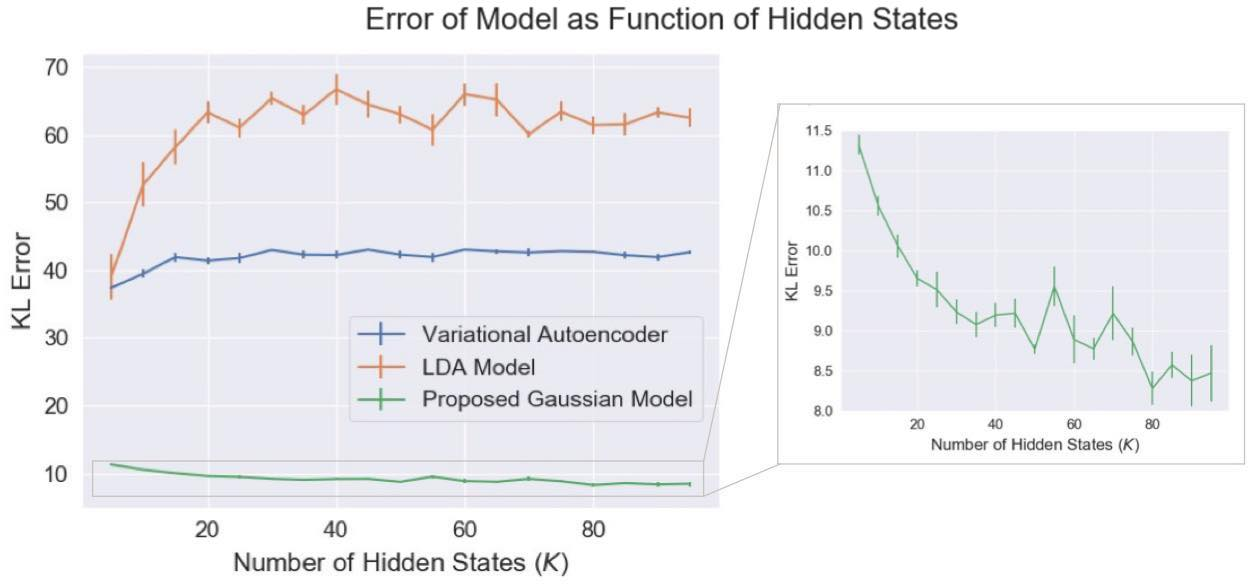
\includegraphics[width=0.9\linewidth]{figures/kl_error.jpg}
    
    \caption{Plots of the $KL$ errors for the proposed model and other models. Right: A plot of the error for just our GMM-based model as a function of hidden state size. Left: A comparison of our model with the two baseline models. The parameter $K$ in the discrete models (LDA and ours) is simply the number of possible hidden state values, whereas for the VAE, it represents the dimension of the latent space.}
    \label{fig:kl_plot}
\end{figure*}

In this section, we describe the data used to train the models presented in Section~\ref{section:background} and how we evaluated them during training. 

\subsection{Data}

We use 18 years of course enrollment data from a large private university in the United States. The data was given in the form of 2.15 million anonymized enrollment records with fields for course name and student major. Importantly, this dataset included not only the enrollment data of full-time students but also part-time and summer school students who were removed before the model was trained. 

Figure~\ref{fig:data_statistics} shows two basic visualizations of the data after removal of part-time students. There are at least two notable takeaways from these plots. First, despite rapid changes in the distribution of sub-school\footnote{These are the broadest partitions of the university which undergraduates commonly take classes in.} enrollments in the first few years of the data, the proportion of enrollments in each school remains relatively stable through most of the data. We use this fact to aggregate over time without explicitly modeling the changes in enrollments patterns. Second, the fact that the number of courses taken can be fit well with a Gaussian shows that enrollment patterns are not intensely multi-modal and thus the assumptions of probabilistic model are very plausible.

In order to learn the parameters of our model, we created training data by aggregating student enrollments per-year and encoding them in the $-1/1$ scheme described in Section~\ref{section:latent-variable-models}. With this data, we train a sequential model of enrollments per major. This step was not strictly necessary and student major could have been modeled latently, but as most of our motivating queries are made at the level of a department, this did not feel like a sacrifice. The results presented here are from models of the 4-year undergraduate degree programs in Computer Science and Math. These were the majors most familiar to the authors, but the same analysis could be carried out on any other major. 

As most of the resulting matrices were of dimension $(n,m)$ with $m > 10^3$, we additionally performed dimensionality reduction by removing classes that had less than 10 overall enrollments by all students of the major over the entire time period. This step also acted as a form of denoising as the produced enrollments tended to be less correlated with the others. 

To make the course codes of classes easier to interpret, we gave them descriptive short names to convey their content succinctly. For example, as per convention, CS1 and CS2 correspond to the introductory computer science classes. Similarly, courses with prefix ``Alg'' or ``AI'' correspond to algorithms or artificial intelligence classes respectively. A full list of course codes and their respective course descriptions can be found in Appendix \ref{app:course_descriptions}.

\subsection{Training and Selection}

Because our model approximates a discrete distribution with a real-valued one, validation with log-likelihood becomes difficult; the hold-out data represents an extremely collapsed subset of the model's support. This mismatch leads to often monotonically decreasing standard log-likelihood metrics. Here we present an alternative metric that can be used to gauge progress during training and compare models when selecting their final parameters. 

We can avoid the detrimental effects of the real-valued relaxation by directly comparing samples from our model, which are discretized, with hold-out data. More specifically, we can compare the empirical enrollment distributions in samples from our model and the distributions of the hold-outs. Let $p^t_j$ be the probability that class $j$ is taken by any given student in the hold-out data, and $p^s_j$ be the corresponding probability in the samples. We take as our error, $E(p^t,p^s)$ with 
\begin{align*}
 E(p^t,p^s) 
 &= \sum_j \infdiv{p^t_j} {p^s_j} \\
 &= - \sum_j p^t_j \log \left( \frac{p^s_j}{p^t_j} \right) + (1 - p^t_j) \log \left(\frac{1-p^s_j}{1 - p^t_j} \right)
\end{align*}
This is precisely the KL divergence between the mean field approximations of the two distributions. In this context, however, it is simply a metric we can use to estimate of the distance between the distribution of our model and the distribution of the data. 

When training a model, we can use this metric to determine hidden state size i.e. the number of discrete values any hidden variable, $h$, can take. This decision is inherently a trade-off between accuracy and computational efficiency. Increasing the size of the hidden states increases the ability of the model to fit the data, but the time required to perform inference scales quadraticly. As we increase the complexity of the model, we also increase the chances of the model overfitting, resulting in poor generalization. In practice, we found that the CMM model became intractable to train before it was expressive enough to overfit the training data. Figure~\ref{fig:kl_plot} shows a plot of the error as a function of hidden state size for our proposed model as well as two comparison models. By looking at the ``elbow'' of the plot, we can identify a reasonable hidden state size that balances accurate modeling of the distribution with computation complexity.

\section{Evaluation}
\label{section:evaluation}



In Figure~\ref{fig:kl_plot} we compare the performance of our model on \textit{hold-out data} relative to baseline models described in Section~\ref{section:baselines}. We also include a direct comparison of the best performance for each model in Table~\ref{tab:kl_table}. 

In Figure~\ref{fig:kl_plot} we can see that our proposed model outperforms the two baselines across the board. It is also evident that the two baselines suffer from bad generalization as the complexity of the model increases. In the case of the VAE, this degradation in performance is due to overfitting made possible by the large hypothesis space of the model. These models were trained adaptively according to performance on the validation set (further described in Appendix \ref{app:VAE_details}) and thus are not simply underfitting due to increase training complexity. The LDA model, on the other hand, is more likely experiencing a degradation in performance because of the naive uniform prior over topic distributions. As hidden state size increases, this assumption can become a handicap that causes the model to draw more heavily from uncommon courses. 

\begin{table}
    \centering
    \begin{tabular}{|c|c|}
    \hline
    Model & KL Error \\
    \hline
    LDA-based Model & 39.8 \\
    Deep Generative Model & 35.5 \\
    Our Gaussian Model & \textbf{7.1} \\
    \hline
    \end{tabular}
    \caption{A direct comparison of the best performance from each model on hold-out data}
    \label{tab:kl_table}
\end{table}


\subsection{Visualizing Hidden Variables}

Beyond using the loss function defined with KL divergence, we can also examine the hidden states of a trained model to validate the learning process. In particular, we can investigate whether the hidden space captures semantically meaningful categories. Figure~\ref{fig:gmm_clusters} shows a visualization for our model trained on CS majors. The clusters in the grid correspond to required courses for three different concentration within the major\footnote{These requirements were taken from the department website: \url{https://exploredegrees.stanford.edu/schoolofengineering/computerscience}.}, and the color shows the most likely latent state assigned by the model to each course. As we can see, courses within the same concentration are assigned strikingly similar latent states by the model, suggesting that the model captures a semantically meaningful notion of the different concentrations in its hidden state.  This result is especially compelling because the model has no access to supervision in the form of listed degree requirements. Therefore, if there are unknown correlations in course enrollments---for example many AI and biology courses taken together---this model could bring these patterns to the fore, allowing administrators an insight into possible ways to improve their degree concentrations.

\begin{figure}[h]
    \centering
    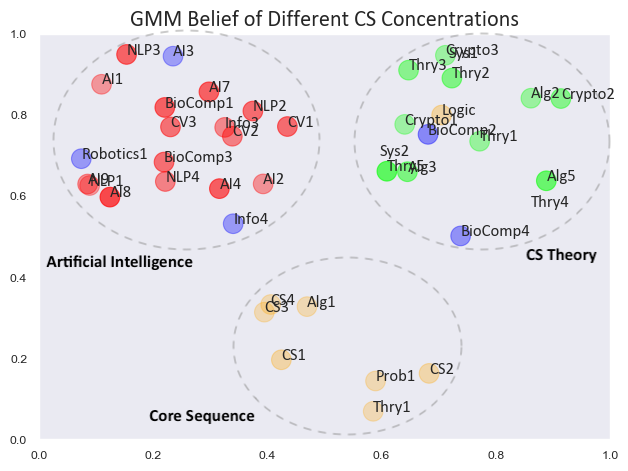
\includegraphics[scale=0.5]{figures/gmm_clusters.png}
    \caption{A visualization of the semantic meaning captured by the latent space of the model. Coloring corresponds to the hidden state most strongly associated with the class. We can see that the hidden states correspond strongly with the required courses for a given concentration. Translucency corresponds to the confidence of the model in its estimate. The full course descriptions can be found in Appendix \ref{app:course_descriptions}.}
    \label{fig:gmm_clusters}
\end{figure}

\section{Applications}
\label{section:applications}

In this section we present results from two different experiments performed with our proposed model. These applications demonstrate only a fraction of the model's scope, but show its power to provide insights.

\subsection{Quantifying Enrollment Likelihood}

One of the useful applications made simple by our generative model is in quantifying enrollment likelihood. A model trained on student enrollments will approximate the distribution of the training data. Thus if we evaluate the likelihood of a new student's enrollments given the model, we can get a sense of how this student differs from the training examples. Taking this principle to its extreme, we can train a model for each student on every other student's enrollments, allowing us to model exactly how much each particular student varies from the typical. 

Figure~\ref{fig:likelihistogram} shows a histogram of the log-likelihood assigned to each undergraduate student in the computer science department using this process. The far left of the histogram contains students whose enrollments are highly atypical, and as we move right these students become less ``surprising" to the model. Most students fall within the middle range, making them neither highly unusual nor cookie-cutter.

By examining the classes taken by students who fall within each region of the histogram, we see that the model captures at least two meaningful axes of variance. Firstly, it recognizes that it is rare for students to take a very diverse set of courses spanning many academic subjects. This insight is demonstrated in Figure~\ref{fig:piecharts}, which shows the average coursework for each type of student. The second insight that the model captures is the spectrum of ambition. More specifically, the model places very low probability on the small subgroup of students that take up to 30 computer science classes and places high probability on taking just the core requirements of the degree\footnote{We can identify this trend by looking at the exact classes that are most commonly taken by these students. For high probability students, these courses are the core requirements.}. Additionally, atypical students take about 20 more courses than their counterparts during their time in school. 

\begin{figure}
    \centering
    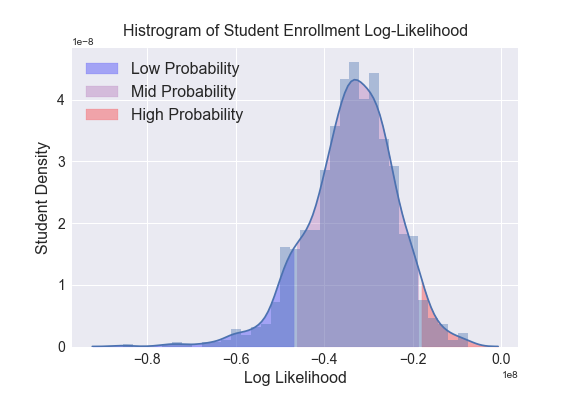
\includegraphics[scale=0.4]{figures/loglikelihood_hist.png}
    \caption{\label{fig:likelihistogram} Histogram of log-likelihoods for each student assigned by model trained on all other students. The three subpopulations of students discussed are highlighted in separate colors.}
\end{figure}

\begin{figure}[h]
    \centering
    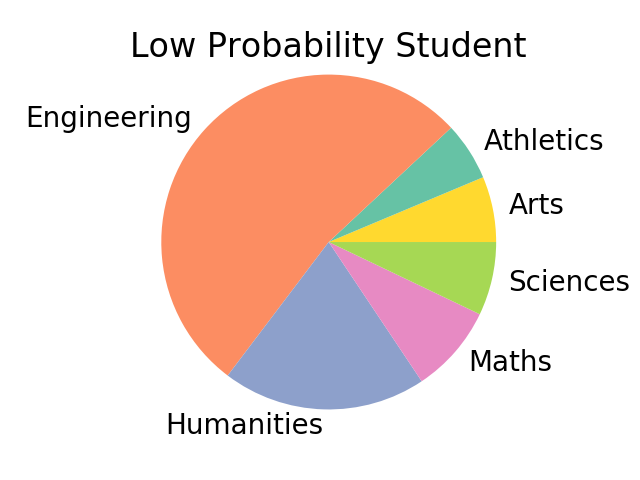
\includegraphics[scale=0.20]{figures/lowpie.png}
    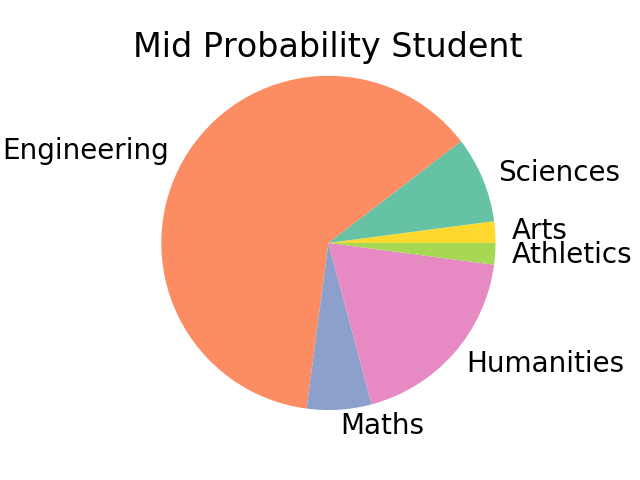
\includegraphics[scale=0.20]{figures/midpie.png} \\
    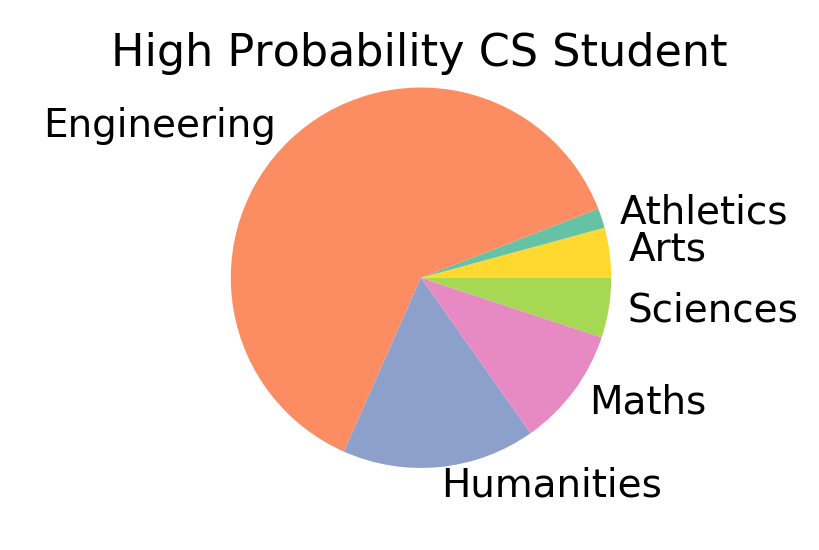
\includegraphics[scale=0.20]{figures/highpie.png}
    \caption{\label{fig:piecharts} Pie charts representing the difference between enrollment patterns captured by the model. Sections correspond to the average number of courses taken in a academic subject by the average student in the respective probability range.}
\end{figure}

\subsection{Understanding Paths}
\label{section:understanding-paths}
   
\begin{figure*}[h!]
    \centering
    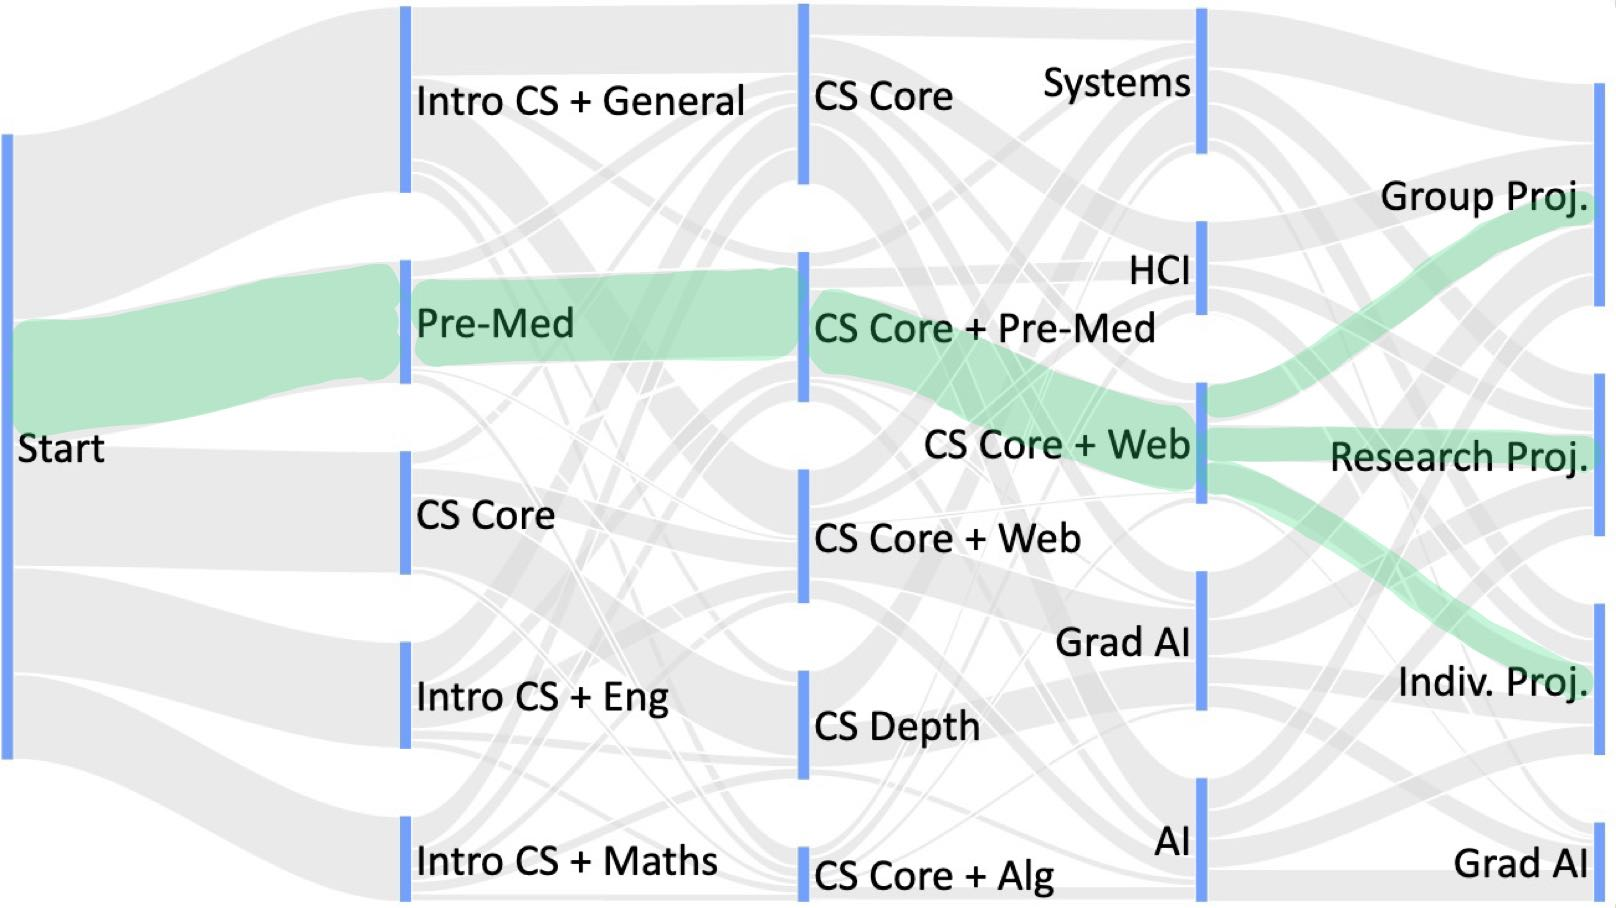
\includegraphics[width=0.45\linewidth]{figures/premed_highlight.jpg} 
    \qquad
    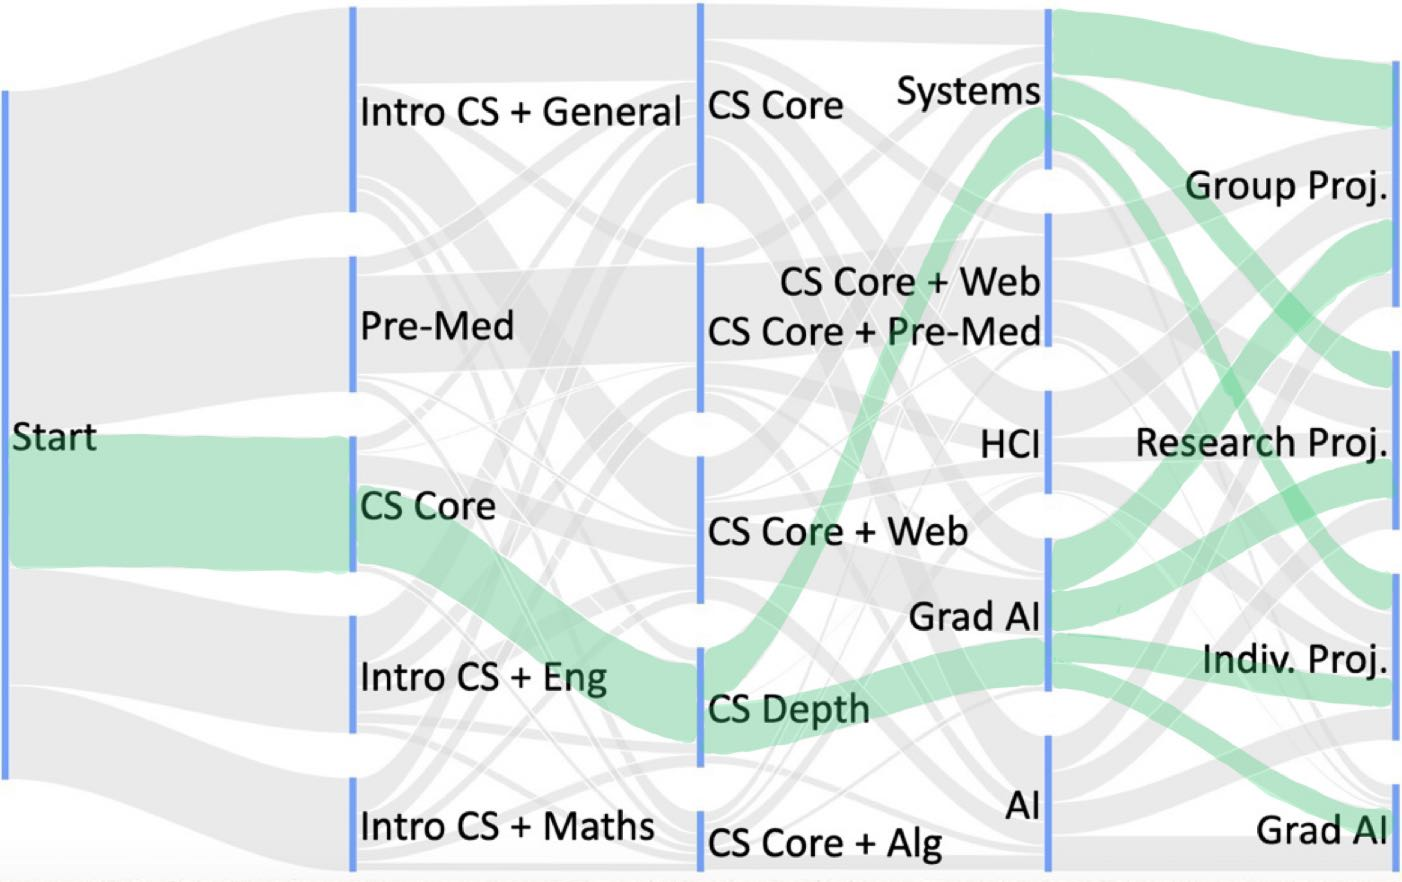
\includegraphics[width=0.41\linewidth]{figures/systems_highlight.jpg}
    % 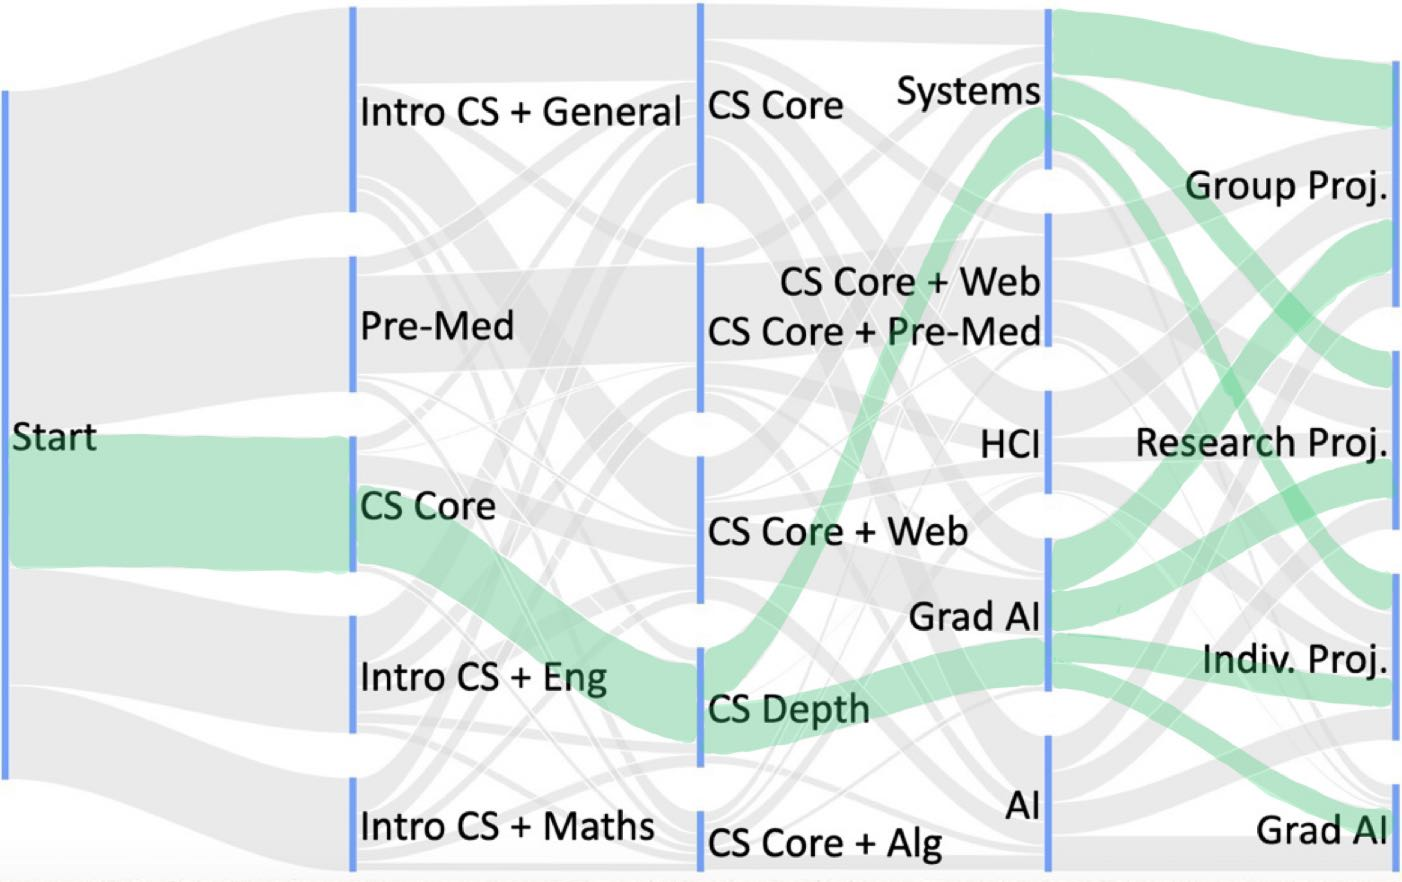
\includegraphics[width=0.48\linewidth]{figures/systems_highlight.png} 
    \caption{\label{fig:cs_sankeys} Two shadings of the same Sankey diagram constructed from the CMM trained on CS undergraduate enrollments. Top: A common path taken by students engaging in pre-med requirements is highlighted in blue. Bottom: A common path for students committed to in-depth study of computer science is highlighted.}
\end{figure*}

Perhaps the most unique capability of the model presented here is the ability to analyze sequences of enrollments, from inferring likely paths between X and Y, to uncovering unspoken student strategies. We can display this visually using Sankey diagrams in which the width of the line between adjacent segments is proportional to the transition probability between the corresponding hidden states in the model. Figure~\ref{fig:cs_sankeys} shows this style of Sankey for CS students. In this diagram, we can note the two types of paths highlighted in the diagram. The first of these captures students who were actively taking the pre-medical requirements freshman and sophomore year. These same students were subsequently much more likely to take depth courses later and were more likely to focus on web development of information systems in their depth courses. We can contrast these students with the students that are highly committed to the CS major and its core classes starting freshman year. These students are much more likely to enroll in depth classes by their sophomore year and are predisposed towards the systems and AI concentrations within the major.
   
As an additional example, we also provide a Sankey diagram for undergraduate students of the Math department in Appendix \ref{app:math_sankey}.
\\
   
\section{Discussion}

Before proceeding to a discussion of future work, we briefly offer context for the probabilistic model we have put forth. In particular, we link the applications we showed in Section~\ref{section:applications} with prior work in the educational literature. 

In recent years, education researchers have discussed the importance of a pathways focused educational system. In \cite{bailey2015redesigning, scott2011shapeless}, Bailey et al. call
for a change in how colleges organize course
offerings. Rather than presenting a cafeteria-style, bewildering
choice of courses, they recommend ``guided pathways'' through the
course offerings. The authors argue that rather than limiting choice,
the result will be educationally coherent programs that will help
students attain a degree faster, and at lower cost.

Rachel Baker \cite{Baker2018} builds on Bailey's work, and suggests
``meta-majors'' for simplifying choice without curtailment. These
artifacts would be combinations of existing majors into larger
coherent units. She proposes the use of social network analysis
techniques to discover opportunities for agglomeration of current
majors.

The creation of guided pathways naturally requires personal
participation from experts in the various academic domains. However,
large data sets of past student enrollments can also inform pathway
design. For example, some courses may be de facto prerequisites for
other courses, even though that fact is not reified in the
corresponding departments' listings. Similarly, ``odd'' delays in taking
particular courses, or unexplained detours in course selection can be
symptoms of unintended scheduling artifacts. The inference capability
of our work, along with appropriate visualizations could help illuminate
such anomalies.

With respect to this point, Armstrong and Hamilton \cite{armstrong2013paying} conducted a five year interview study with students in a large institution of higher learning. The authors expose how strongly the most highly visible, oft trodden course choice paths impact outcomes for students. Some paths can be shown to lead towards low college debt and rich professional choices. Others do not fill reasonable expectations of a worthy college education.

If one were to attempt mitigation of realities described in Armstrong and Hamilton's work, existing paths need to be exposed. Alternative
paths need to be envisioned, and maybe simulated. Approaches such as we present here, as well as alternative analytic approaches we point to in Section~\ref{section:related-work} are prerequisites for a thoughtful evaluation of current practice.

\section{Conclusion \& Future Work}

In this paper, we have presented a new probabilistic model of enrollments that is capable of capturing joint relationships between course enrollments, while also allowing for powerful inference queries. We have demonstrated the soundness of this model and shown how it could be used as a tool for administration, course planning, and education research. The capabilities of this model are, in most cases, a superset of those offered by others, and the model can be trained easily in an unsupervised manner, with little intimate knowledge of the institution. 

There are, however, a few notable drawbacks of our approach. First among these is the strictly Markovian nature of the model. Although this assumption allows us to easily learn the parameters of the model, in practice the enrollments observed at one timestep will impact those sampled at the next timestep. These effects are to some extent modeled by the latent structure of the model, but an alternative approach could involve sacrificing the Markov assumption in order to capture more of these effects with a smaller number of hidden states. Our approach, on the other hand, is effective with less training data than, for example, a recurrent neural net. Our method is therefore more easily deployed for institutions smaller than ours.

Another limitation of the current work is the smoothing step we use to reduce the dimensionality of the data. Though in most cases this reduction is benign, it can in some cases erase patterns that exist in the data but which would only be measurable in aggregate across courses. Take for example the enrollment of engineering students in many different small humanities seminars. No individual seminar witnesses significant enrollments, but in aggregate they create a discernible pattern. Such effects can be ignored by a model that focuses on class enrollments on a per class basis, not per subject or department, as our does. This problem could be easily addressed by a hierarchical latent space that allows the model to learn aggregates trends across small groups of classes. One drawback of the increase in complexity, however, would be a corresponding decrease in interpretability. 

Lastly, we would like to note the potential for future work that links data we used here with other rich information sources such as demographic and grade data. We currently model joint enrollments of course enrollment, assuming that enrollments are influenced by the latent hidden state. Given socioeconomic, demographic, or grade data, we could trivially alter the model to jointly model enrollments as well as these factors. Such a model could meaningfully identify the differences between course trajectories of students with different backgrounds, providing insights into how policies could be tuned to benefit underprivileged and underrepresented groups. Given that we were able to learn a semantically meaningful representation with enrollment data alone, it is easy to imagine how much more powerful the model could become with access to additional information sources---not only in its ability to recreate the empirical features of the distribution but also in the potential of the model to offer insights that are meaningful to students and staff. 

%ACKNOWLEDGMENTS are optional
\section{Acknowledgments}

We would like to acknowledge the support of the Stanford CartaLab for guiding the research and organising the acquisition of data used in this work.  

% The following two commands are all you need in the
% initial runs of your .tex file to
% produce the bibliography for the citations in your paper.
\bibliographystyle{abbrv}
\bibliography{sigproc} 


\balancecolumns
\appendix

\section{Course Descriptions}
\label{app:course_descriptions}

The following table shows the course descriptions for all the course codes used in this paper:

% TODO: add these
\textbf{Removed for anonymised submission}.

\section{Contextual Mixture Model Details}
\subsection{EM Parameter Update}
\label{app:em_update}


\begin{figure*}[h]
    \centering
    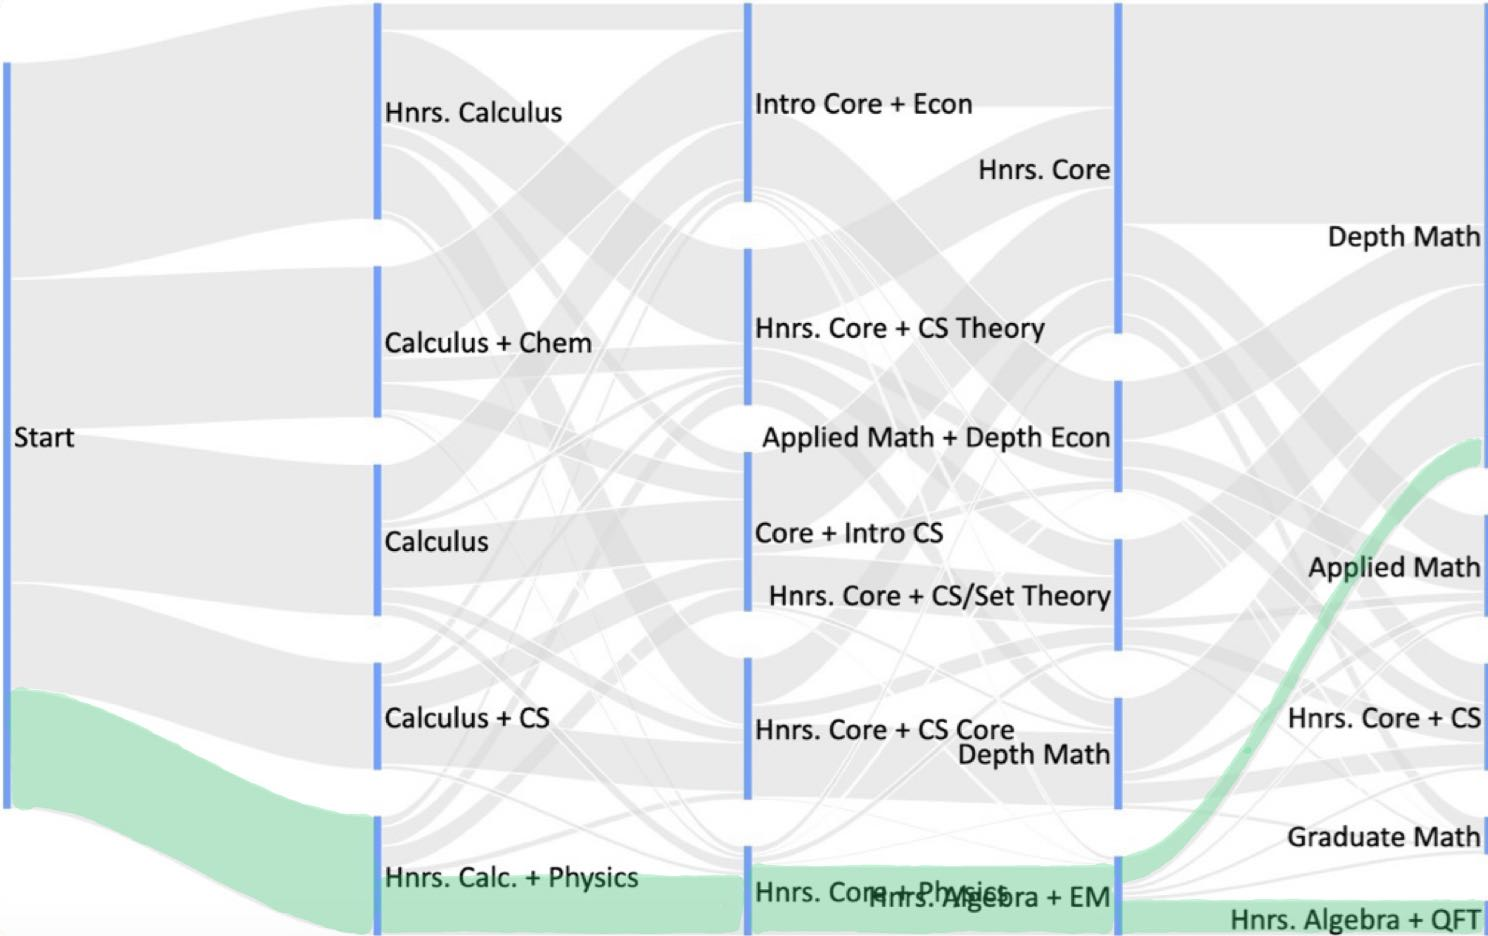
\includegraphics[width=0.48\linewidth]{figures/physics_highlight.jpg}
    \quad 
    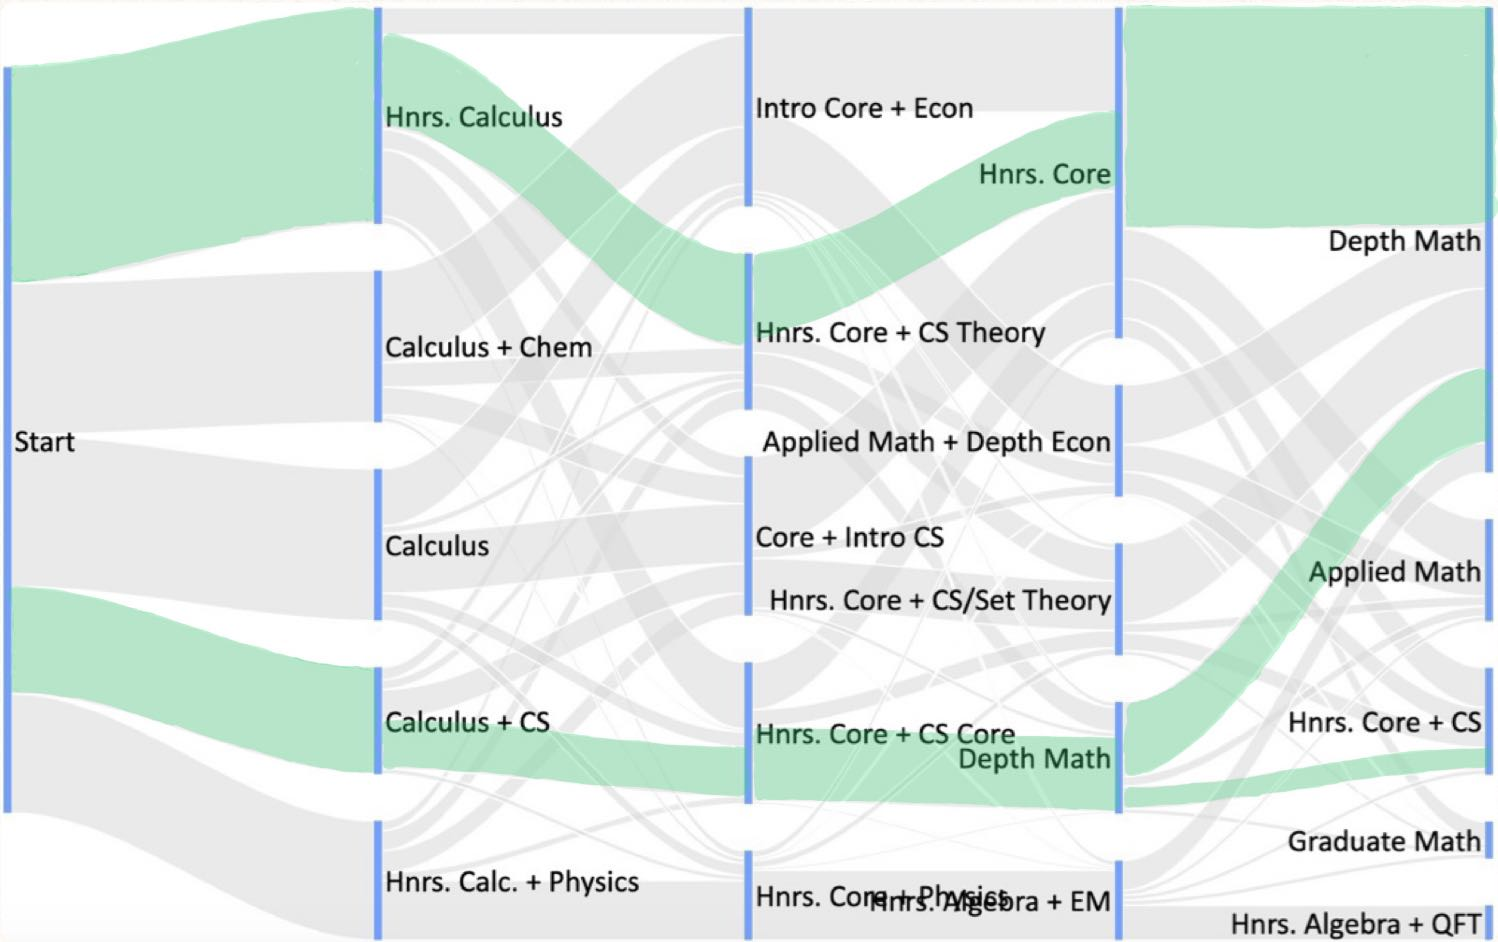
\includegraphics[width=0.48\linewidth]{figures/math_highlight.jpg}
    \caption{A Sankey diagram showing latent pathways for undergraduate math students. Left: A pathway for students that either double-major in physics and Math or just heavily augment their math education with physics courses. Right: Two different pathways are highlighted--one focusing on applied math and one with more focus on theoretical topics.}
    \label{fig:math-sankey}
\end{figure*}

For the Contextual Mixture Model described in Section \ref{section:cmm}, we have the following E and M steps:

\textbf{E Step:}
We calculate
\begin{align*}
Q(h^t \mid X_i) &= \frac{\alpha_k(t) \beta_k(t)}{\sum_k \alpha_k(t) \beta_k(t)} \\
Q(h^t, h^{t+1} \mid X_i) &= \frac{\alpha_k(t) \phi^t_{k k'} \mathcal{N}(X_{t+1};\mu_{k'},\Sigma_{k'}) \beta_{k'}(t)}{\sum_k \sum_{k'} \alpha_k(t) \phi^t_{k k'} \mathcal{N}(X_{t+1};\mu_{k'},\Sigma_{k'}) \beta_{k'}(t)} \\
\end{align*}
with 
\begin{align*}
\alpha_k(0) &= \theta_k \mathcal{N}(X^0; \mu_k^0, \Sigma_k^0)  \\
\alpha_k(t+1) &= \mathcal{N}(X^{t+1}; \mu_k^{t+1}, \Sigma_k^{t+1}) \sum_{k'} \alpha_{k'}(t) \phi^t_{kk'}
\end{align*}
and
\begin{align*}
\beta_k(T-1) &= 1\\
\beta_k(t) &= \sum_{k'} \beta_{k'}(t+1) \mathcal{N}(X^{t+1}; \mu_{k'}^{t+1}, \Sigma_{k'}^{t+1}) \phi^t_{kk'}
\end{align*}

\textbf{M Step:}
Using the probabilities calculated in the E step, we can find parameter estimates maximizing the evidence lower bound as 
\begin{align*}
\theta &= \frac{1}{N} \sum_i Q(h^0 \mid X_i) \\
\phi^t &= \frac{\sum_i Q(h^t, h^{t+1} \mid X_i)} {\sum_i Q(h^t \mid X_i)}\\
\mu_k^t &= \frac{\sum_i Q(h^t_k \mid X_i) X_i^t} {\sum_i Q(h_k^t \mid X_i)}\\
\Sigma^t_k &= \frac{\sum_i Q(h^t_k \mid X_i) (\mu_k^t - X_i^t)(\mu_k^t - X_i^t)^T} {\sum_i Q(h_k^t \mid X_i)}
\end{align*}

\subsection{Gradient Descent Objective}

Here we directly calculate the log-likelihood of the data by marginalization over the hidden states, $h^t$. This amounts to calculating
\begin{align*}
ll(X_i^t ; \, &\theta,\phi^{1:T},\mu^{1:T},\Sigma^{1:T}) \, = \\
& \sum_{h^{0:T}} \left[ \log \theta_{h^0}^0 + \sum_{t=1}^T \log \mathcal{N}(X^t_i;\mu_{h^t}^t,\Sigma_{h^t}^t) + \log 
\phi_{h^{t-1}h^t}^{t-1} \right]
\end{align*}
by sum-product message passing down the hidden Markov chain. This is equivalent to breaking the sum $\sum_{h^{0:T}}$ into its constituent sums $\sum_{h^0} \sum_{h^{1}} ... \sum_{h^T}$. 

\section{VAE Model Details}
\label{app:VAE_details}

\textbf{Encoder/Decoder Network:} \\
The architecture of encoder network is a feed-forward network with the following layer sizes:
\begin{center}
\begin{tabular}{|c|c|}
\hline
Layer & Size \\
\hline 
Input Layer & $\approx 1000$ \\
Hidden Layer 1  & 400 \\
Hidden Layer 2 & $K$ ($5 \leq K \leq 100$) \\
\hline
\end{tabular}
\end{center}
The decoder network is the inverse architecture. We use relu non-linearities and dropout between hidden layers. The network was trained on reconstruction loss and KL divergence with L2 regularization--using the Adam optimizer. The optimization parameters are shown in the table below:
\begin{center}
\begin{tabular}{|c|c|}
\hline
Parameter & Value \\
\hline 
Learning Rate & $5e$-$3$ \\
Weight Decay  & $1e$-$2$ \\
Regularization Weight & $1e$-$3$ \\
Dropout Rate & 0.5 \\
\hline
\end{tabular}
\end{center}
We used a validation holdout set to decide when to perform early stopping during training. We measured performance on the validation set every 50 epochs using the KL divergence. If the measured number increased two sets of 50 epochs in a row, we ended training. This approach prevented drastic overfitting on the training set. 

\section{Math Student Sankey Diagram}
\label{app:math_sankey}

Figure~\ref{fig:math-sankey} shows a Sankey diagram in the style described in Section~\ref{section:understanding-paths} for undergraduate students in the math department. For clarity, we highlight a few meaningful paths exhibited by students in this degree program. 

\end{document}
